\documentclass[12pt, a4paper]{article}

\usepackage{lastpage}
\usepackage{mathtools}
\usepackage{xltxtra}
\usepackage{libertine}
\usepackage{amsmath}
\usepackage{amsthm}
\usepackage{amsfonts}
\usepackage{amssymb}
\usepackage{enumitem}
\usepackage{xcolor}
\usepackage[left=1.5cm, right=1.5cm, top=2cm, bottom=2cm, bindingoffset=0cm, headheight=15pt]{geometry}
\usepackage{fancyhdr}
\usepackage[russian]{babel}
% \usepackage[utf8]{inputenc}
\usepackage{catchfilebetweentags}
\usepackage{accents}
\usepackage{calc}
\usepackage{etoolbox}
\usepackage{mathrsfs}
\usepackage{wrapfig}

\providetoggle{useproofs}
\settoggle{useproofs}{false}

\pagestyle{fancy}
\lfoot{M3137y2019}
\rhead{\thepage\ из \pageref{LastPage}}

\newcommand{\R}{\mathbb{R}}
\newcommand{\Q}{\mathbb{Q}}
\newcommand{\C}{\mathbb{C}}
\newcommand{\Z}{\mathbb{Z}}
\newcommand{\B}{\mathbb{B}}
\newcommand{\N}{\mathbb{N}}

\newcommand{\const}{\text{const}}

\newcommand{\teormin}{\textcolor{red}{!}\ }

\DeclareMathOperator*{\xor}{\oplus}
\DeclareMathOperator*{\equ}{\sim}
\DeclareMathOperator{\Ln}{\text{Ln}}
\DeclareMathOperator{\sign}{\text{sign}}
\DeclareMathOperator{\Sym}{\text{Sym}}
\DeclareMathOperator{\Asym}{\text{Asym}}
% \DeclareMathOperator{\sh}{\text{sh}}
% \DeclareMathOperator{\tg}{\text{tg}}
% \DeclareMathOperator{\arctg}{\text{arctg}}
% \DeclareMathOperator{\ch}{\text{ch}}

\DeclarePairedDelimiter{\ceil}{\lceil}{\rceil}
\DeclarePairedDelimiter{\abs}{\left\lvert}{\right\rvert}

\setmainfont{Linux Libertine}

\theoremstyle{plain}
\newtheorem{axiom}{Аксиома}
\newtheorem{lemma}{Лемма}

\theoremstyle{remark}
\newtheorem*{remark}{Примечание}
\newtheorem*{exercise}{Упражнение}
\newtheorem*{consequence}{Следствие}
\newtheorem*{example}{Пример}
\newtheorem*{observation}{Наблюдение}

\theoremstyle{definition}
\newtheorem{theorem}{Теорема}
\newtheorem*{definition}{Определение}
\newtheorem*{obozn}{Обозначение}

\setlength{\parindent}{0pt}

\newcommand{\dbltilde}[1]{\accentset{\approx}{#1}}
\newcommand{\intt}{\int\!}

% magical thing that fixes paragraphs
\makeatletter
\patchcmd{\CatchFBT@Fin@l}{\endlinechar\m@ne}{}
  {}{\typeout{Unsuccessful patch!}}
\makeatother

\newcommand{\get}[2]{
    \ExecuteMetaData[#1]{#2}
}

\newcommand{\getproof}[2]{
    \iftoggle{useproofs}{\ExecuteMetaData[#1]{#2proof}}{}
}

\newcommand{\getwithproof}[2]{
    \get{#1}{#2}
    \getproof{#1}{#2}
}

\newcommand{\import}[3]{
    \subsection{#1}
    \getwithproof{#2}{#3}
}

\newcommand{\given}[1]{
    Дано выше. (\ref{#1}, стр. \pageref{#1})
}

\renewcommand{\ker}{\text{Ker }}
\newcommand{\im}{\text{Im }}
\newcommand{\grad}{\text{grad}}

\lhead{Конспект по матанализу}
\cfoot{}
\rfoot{Лекция 6}

\usepackage[]{graphics}

\begin{document}

\section*{Интегральные суммы}

\begin{definition}
    \textbf{Дробление} отрезка $[a,b]$ это разбиение отрезка на $n$ частей следующим образом:
    $$x_0=a<x_1<x_2<\ldots<x_n=b \quad [x_{i-1}, x_i]$$
\end{definition}

\begin{definition}
    \textbf{Ранг \textit{(мелкость)}} дробления --- длина самого длинного из отрезков дробления:
    $$\tau = \{x_0\ldots x_n\} \quad |\tau|=\max(x_i-x_{i-1})$$
\end{definition}

\begin{definition}
    \textbf{Оснащение} --- множество точек $\{\xi_1\ldots \xi_n\} : \xi_i\in[x_{i-1}, x_i]$
\end{definition}

\begin{definition}
    \textbf{Интегральная сумма} для разбиения $\{x_i\}$, произвольной функции $f$ и оснащения $\{\xi_i\}$ это следующая сумма:
    $$\sum_{i=1}^n f(\xi_i)(x_i-x_{i-1})$$
\end{definition}

Геометрически интегральная сумма интерпретируема следующим образом:

\begin{figure}[!htbp]
    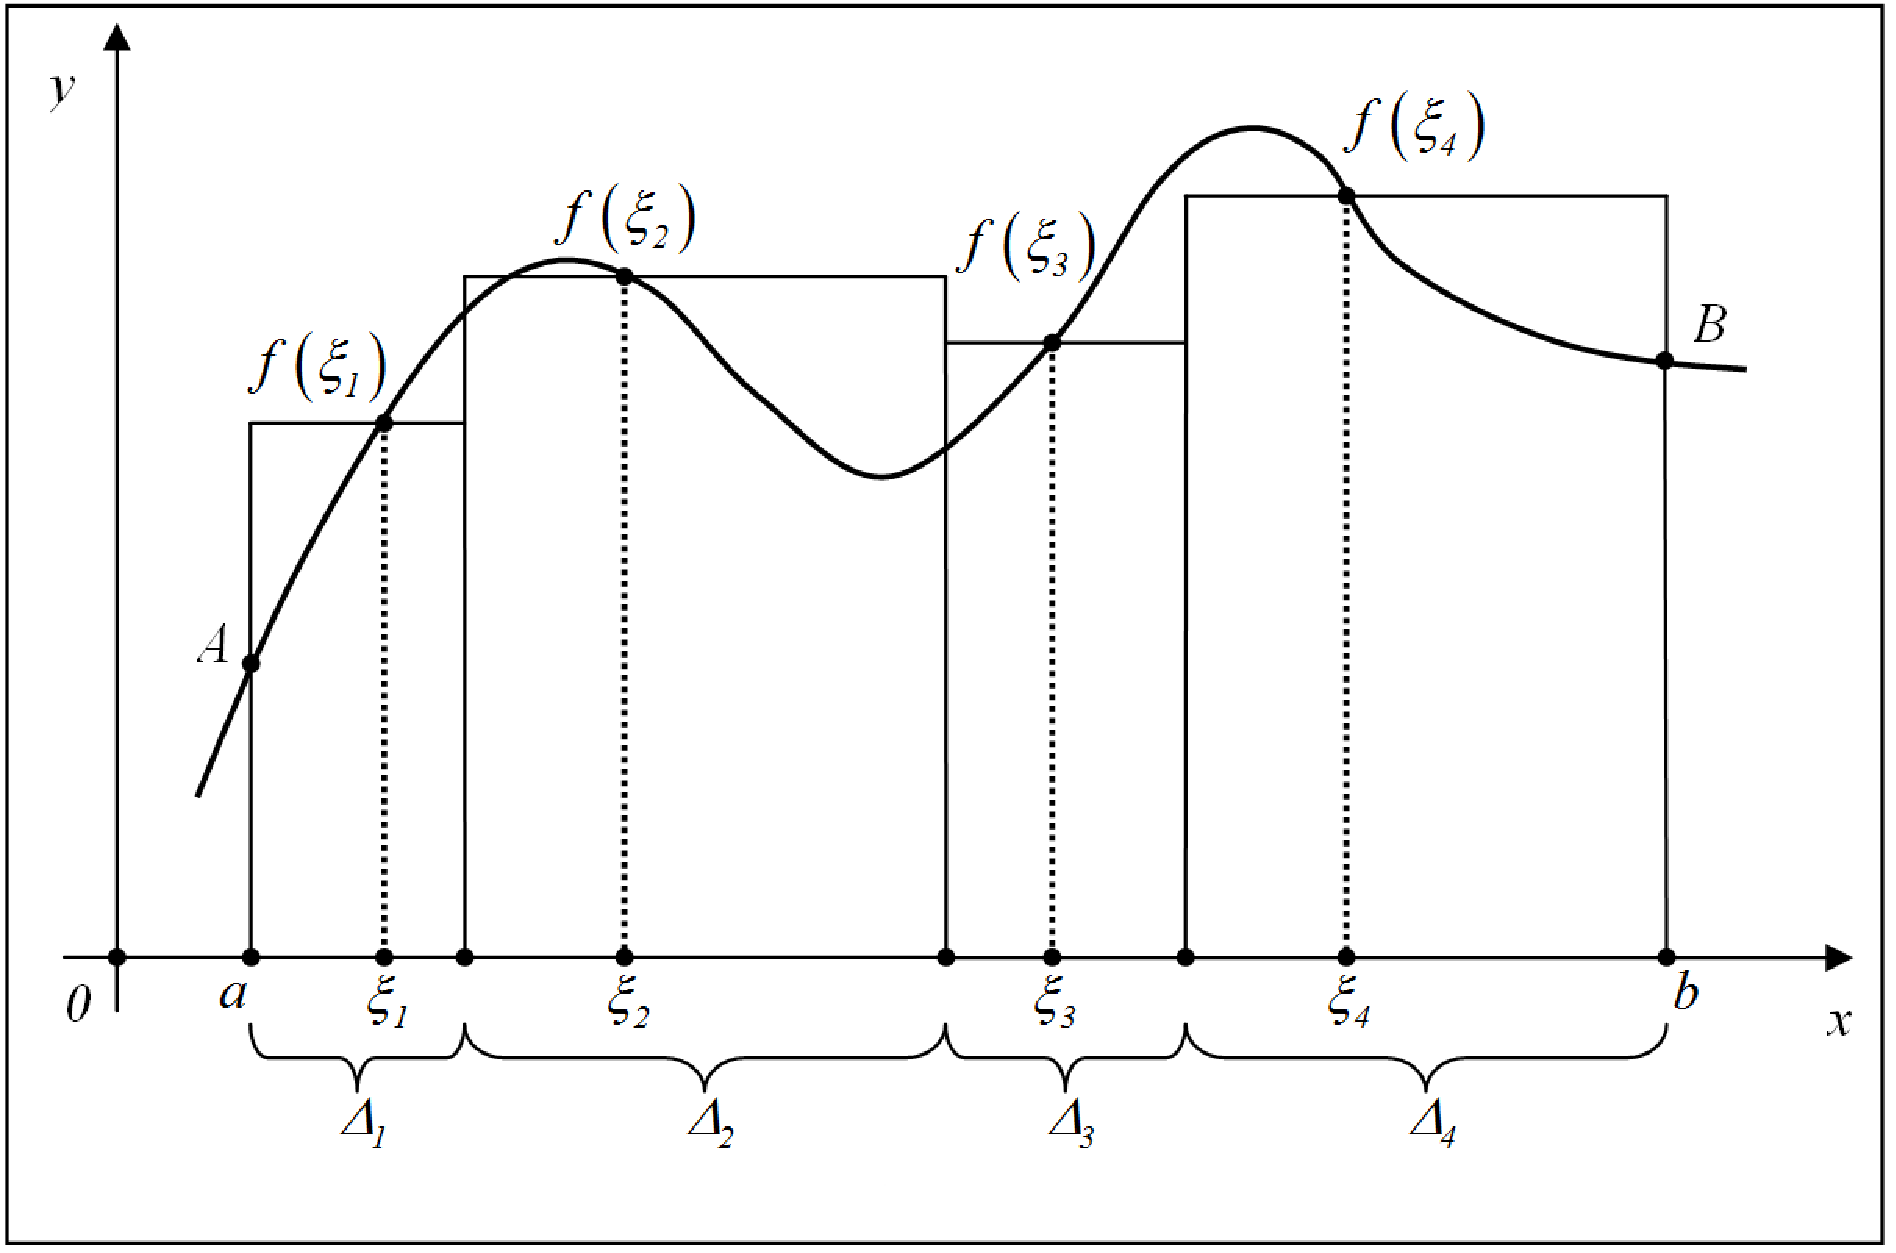
\includegraphics[scale=0.4]{images/riemann-sum.pdf}
    \centering
\end{figure}

\begin{theorem}
    Об интеграле как пределе интегральных сумм.

    %<*обинтегралекакпределеинтегральныхсумм>
    $f\in C[a,b]$
    $$\forall \varepsilon > 0 \ \ \exists \delta>0 \ \ \forall \text{дробление } \tau=\{x_0\ldots x_n\} : |\tau|<\delta \ \ \forall \text{оснащение } \xi_i \quad \left|\int_a^b f(x)dx - \sum_{i=1}^n f(\xi_i)(x_i-x_{i-1})\right| < \varepsilon$$
    %</обинтегралекакпределеинтегральныхсумм>
\end{theorem}
%<*обинтегралекакпределеинтегральныхсумм>
\begin{proof}
    По теореме Кантора о равномерной непрерывности на компакте.

    $[a,b]$ --- компакт, $f$ непрерывна на $[a,b] \Rightarrow f$ равномерно непрерывна на $[a,b]$:
    $$\forall \varepsilon > 0 \ \ \exists \delta > 0 \ \ \forall x, \overline x\in[a,b] : |x-\overline x|<\delta \quad |f(x)-f(\overline x)|<\varepsilon$$
    По двойной бухгалтерии заменим $\varepsilon$ на $\cfrac{\varepsilon}{b-a}$:
    $$\forall \varepsilon > 0 \ \ \exists \delta > 0 \ \ \forall x, \overline x\in[a,b] : |x-\overline x|<\delta \quad |f(x)-f(\overline x)|<\frac{\varepsilon}{b-a}$$
    Разобьем интеграл на части:
    $$\int_a^b f(x)dx=\sum_{i=1}^n \left(\int_{x_{i-1}}^{x_i} f(x)dx\right)$$
    Запишем $(x_i-x_{i-1})$ в виде интеграла $\int_{x_{i-1}}^{x_i} dx$
    $$\left|\int_a^b f(x)dx - \sum_{i=1}^n f(\xi_i)(x_i-x_{i-1})\right|=\left|\sum_{i=1}^n\left(\int_{x_{i-1}}^{x_i} f(x)dx - f(\xi_i)\int_{x_{i-1}}^{x_i} dx\right)\right|=$$
    $$=\left|\sum_{i=1}^n\int_{x_{i-1}}^{x_i}(f(x)-f(\xi_i))dx\right|\leq\sum\left|\int\right|\leq\sum_{i=1}^n\int_{x_{i-1}}^{x_i}|(f(x)-f(\xi_i))dx|\leq \sum_{i=1}^n\int_{x_{i-1}}^{x_i}\frac{\varepsilon}{b-a}dx=$$
    $$=\frac{\varepsilon}{b-a}\sum_{i=1}^n\int_{x_{i-1}}^{x_i}dx=\frac{\varepsilon}{b-a}\sum_{i=1}^n(x_{i}-x_{i-1})=\frac{\varepsilon}{b-a}(b-a)=\varepsilon$$
\end{proof}
%</обинтегралекакпределеинтегральныхсумм>

\begin{remark}
    $f\in C^1[a,b]$; $M:=\max\limits_{x\in[a,b]} |f'(x)|$

    $$|f(x)-f(\overline x)|=|f'(\overline x)(x-\overline x)|\leq M|x-\overline x|$$
\end{remark}

\begin{consequence}
    Равномерное дробление: $x_i=a+\frac{b-a}{n}i; |\tau|=\frac{b-a}{n}$
    $$\int-\sum\leq M(b-a)^2\frac{1}{n}$$
\end{consequence}

\begin{theorem}
    Об интегральных суммах центральных прямоугольников

    $f\in C^2[a,b] \ \ x_0=a<x_1\ldots <x_n=b \ \ \delta=\max(x_i-x_{i-1}) \ \ \xi_i:=\frac{x_{i-1}+x_i}{2}$. Тогда
    $$\left|\int_a^b f-\sum_{i=1}^n f(\xi_i)(x_i-x_{i-1})\right|\leq \frac{\delta^2}{8}\int_a^b |f''|dx$$
\end{theorem}
\begin{proof}
    $$\int_{x_{i-1}}^{x_i} f(x)dx = \int_{x_{i-1}}^{\xi_i} f(x)dx + \int_{\xi_i}^{x_i} f(x)dx = \int_{x_{i-1}}^{\xi_i} f(x)d(x-x_{i-1}) + \int_{\xi_i}^{x_i} f(x)d(x-x_i)=$$
    $$=f(x)(x-x_{i-1})|_{x=x_{i-1}}^{x=\xi_i}-\int_{x_{i-1}}^{\xi_i} f'(x)(x-x_{i-1})dx+f(x)(x-x_{i-1})|^{x=x_{i}}_{x=\xi_i}$$
\end{proof}

% Простейший случай формулы Эйлера-Маклорена

% $m, n\in \Z, f\in C^2[m, n]$. Тогда
% $$\int_m^n f(x)dx=\left(\sum_{i=m}^n\right)' f(i)-\frac{1}{2}\int f ''(x)[x](1-[x])dx$$
% $'$ означает, что крайние слагаемые берутся с весом $\frac{1}{2}$
% \begin{proof}
%     Очевидно.
% \end{proof}

\end{document}